\section{Features Guide}
The following section contains the list of all the allowed operations that the different types of user can perform inside \app. \\
Please note that, due to time reasons, not all the features are currently implemented, but they will be implemented in a short time and this section will be so updated. These features will be marked by a * near their names.

\subsection{Users' types}
The common use of the application will involve different types of users, which can be represented by the following hierarchy, from the one that has fewer permissions (at the top) to the one with the most permissions (at the bottom):
\begin{itemize}
	\item \textbf{View-only user}, also simply called \textbf{viewer}. \\
		  This kind of user can just view the list, without interacting with it. The operations that this kind of user can perform will be marked with an \texttt{[V]} near their name;
	\item \textbf{Common user}, also called \textbf{user}.
		  This kind of user does nothing else than interacting with an already-created list, performing common operations. The operations that this kind of user can perform will be marked with an \texttt{[U]} near their name;
	\item \textbf{Permissions-granted user}, also called \textbf{editor}.
		  This kind of user has all the above permissions, plus he can add or remove items to the list. All the operations that he can perform will be marked with an \texttt{E} near their name;
	\item \textbf{Creator of the list}, also called \textbf{creator}
		  This kind of user is the user that creates a list and so can perform some special actions on it. The operation that this kind of user can perform are marked with a \texttt{[C]} near their name.
\end{itemize}

\newpage
\subsection{[U] Creating a list}
In order to create a list just click on the following button that is present on the right-side bar of the chat.

% Inserire immagine del bottone
\begin{figure}[H]
  \centering 
  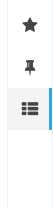
\includegraphics[width=\textwidth]{Sections/3-HowToUse/Images/create_list_button.png}
  \caption{Bubble creation button.}
\end{figure}

This will open the following screen, where you can input all the information that you want about the list, reminding that the only \textbf{required option} is the list's title.

% Inserire immagine schermata inserimento dati lista
\begin{figure}[H]
  \centering 
  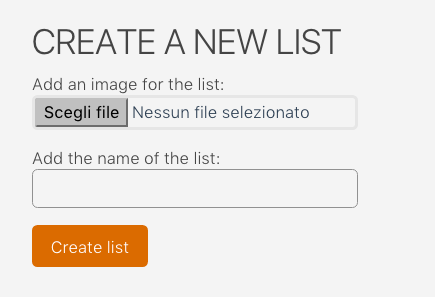
\includegraphics[width=\textwidth]{Sections/3-HowToUse/Images/list_create.png}
  \caption{List information input screen.}
\end{figure}

Once that all the information are input, in order to create the list just click on the \textit{"Create"} button, which will create the bubble as shown below.

% Inserire immagine della bolla creata
\begin{figure}[H]
  \centering 
  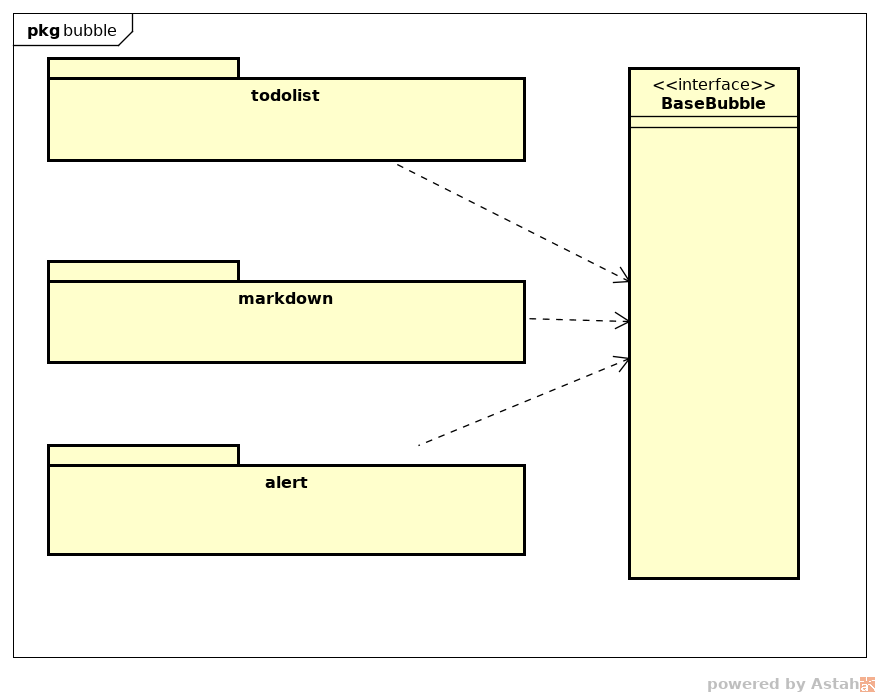
\includegraphics[width=\textwidth]{Sections/3-HowToUse/Images/bubble.png}
  \caption{Created bubble which represents the list.}
\end{figure}
%\subsection{[C] Editing a list *}
In order to edit a list, hover on top of the \termine{bubble} that represents the list and click on the gear icon.

% Inserire immagine delle opzioni che vengono fuori al passaggio del mouse sopra la bolla
\begin{figure}[H]
  \centering 
  
\includegraphics[width=\textwidth]{Sections/3-HowToUse/Images/example.jpeg}
  \caption{Button to show the available list's actions.}
\end{figure}

From the various options that will appear, click on the one with a pencil as the icon.

% Inserire immagine icona di modifica della lista
\begin{figure}[H]
  \centering 
  
\includegraphics[width=\textwidth]{Sections/3-HowToUse/Images/example.jpeg}
  \caption{Icon of the option to edit a list's information.}
\end{figure}

This will open the following screen, where it's possible to change all the information that you want about the list, reminding that the only \textbf{required information} is the list's title, which cannot be empty.

% Inserire immagine schermata dati inseriti
\begin{figure}[H]
  \centering 
  
\includegraphics[width=\textwidth]{Sections/3-HowToUse/Images/example.jpeg}
  \caption{List information editing screen.}
\end{figure}

Once that all the information are input, in order to save the changes, just click on the \textit{"Save"} button which will save the \termine{bubble}'s information.

% Inserire immagine della bolla modificata
\begin{figure}[H]
  \centering 
  
\includegraphics[width=\textwidth]{Sections/3-HowToUse/Images/example.jpeg}
  \caption{Bubble after the information edit.}
\end{figure}
\newpage
\subsection{[E] Adding an item to the list}
In order to add an item to the list, just click on the proper button that is present on the bubble that represents the list itself.

% Immagine della bolla con il bottone per aggiungere un oggetto
\begin{figure}[H]
  \centering 
  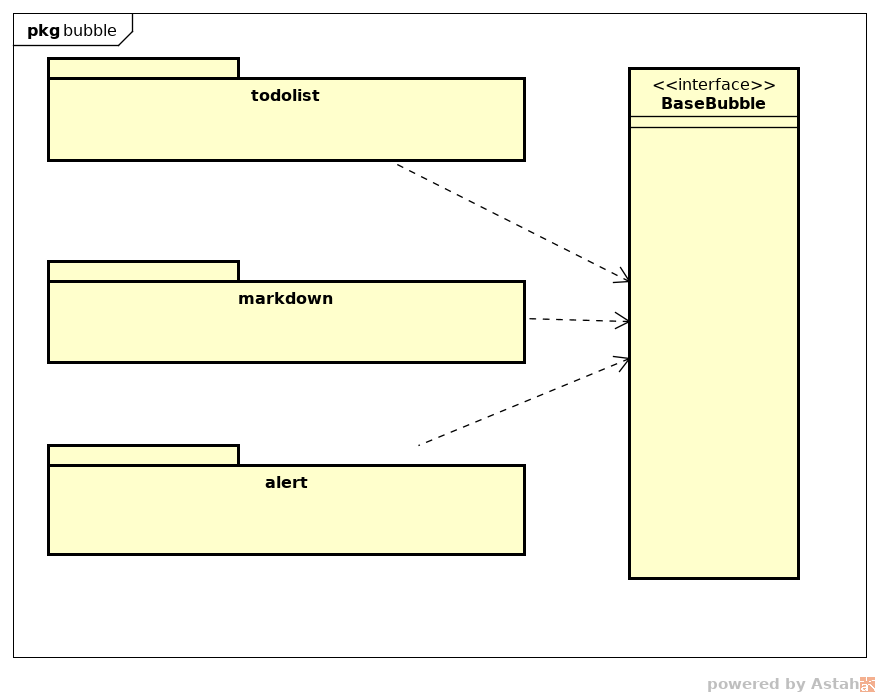
\includegraphics[scale=0.3]{Sections/3-HowToUse/Images/bubble.png}
  \caption{Bubble with the button to add an item inside.}
\end{figure}

This will open the following screen, where you can input all the information about the item that needs to be added to the list. \\

% Immagine della schermata per inserimento dati oggetto
\begin{figure}[H]
  \centering 
  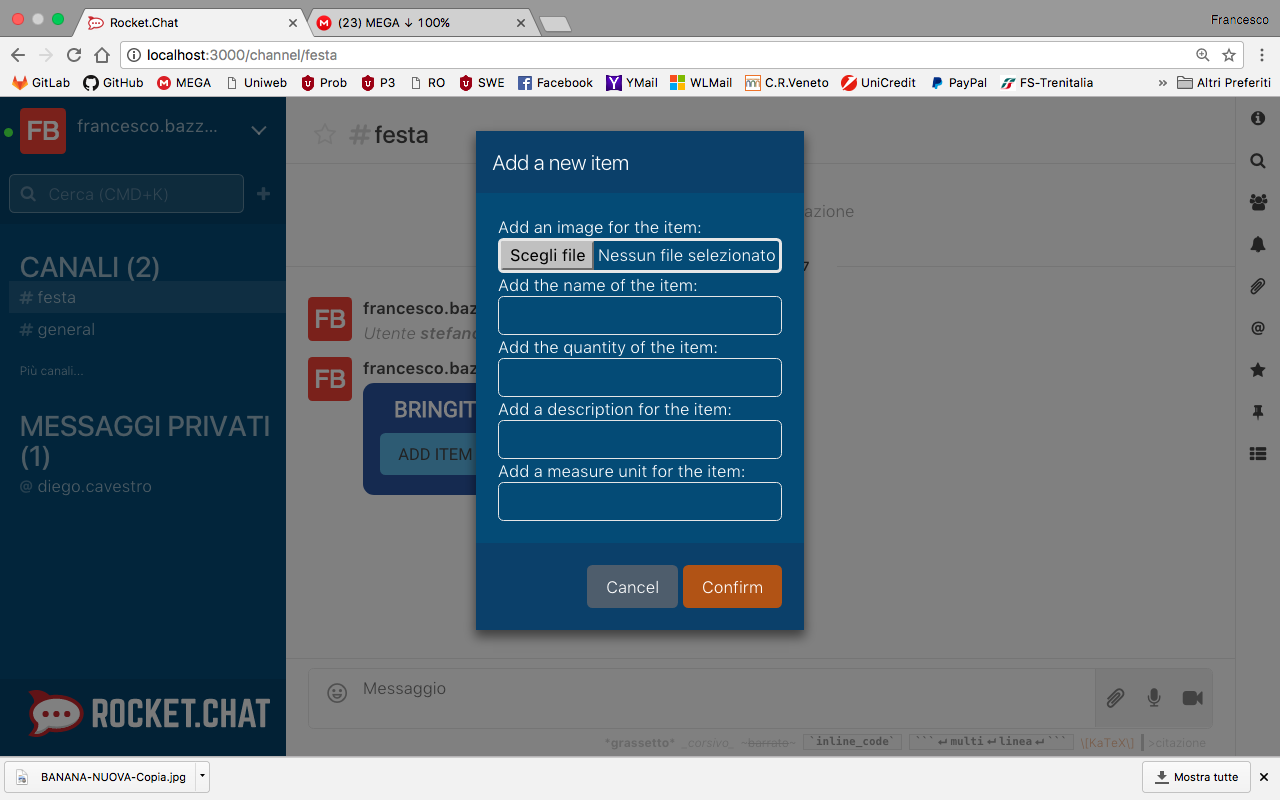
\includegraphics[scale=0.5]{Sections/3-HowToUse/Images/item_add.png}
  \caption{Item information input screen.}
\end{figure}

Once that all the data have been input, in order to add the item just click on the \textit{"Add"} button, which will add the item to the list.

% Immagine della bolla con il nuovo oggetto aggiunto
\begin{figure}[H]
  \centering 
  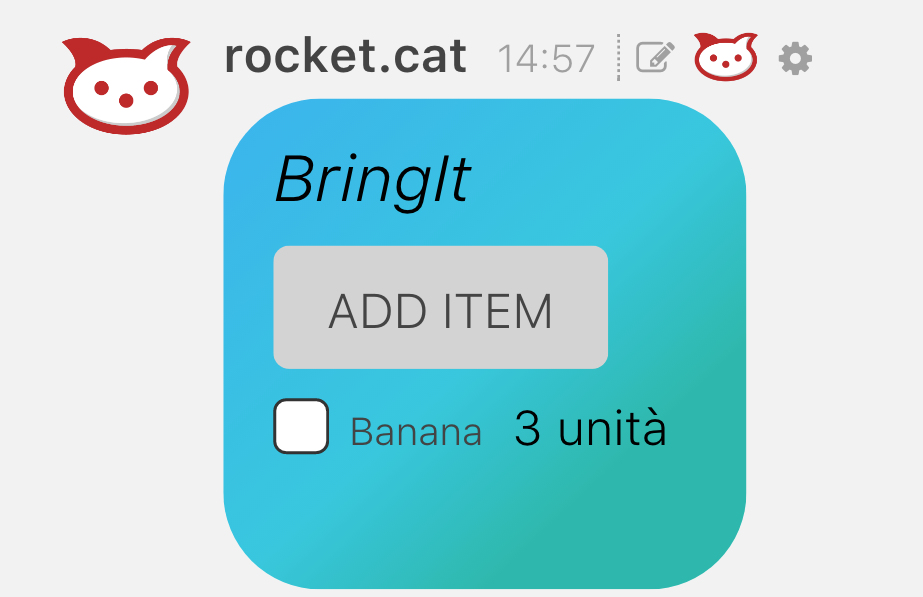
\includegraphics[scale=0.3]{Sections/3-HowToUse/Images/bubble_with_item.png}
  \caption{Bubble with the new item added.}
\end{figure}
%\subsection{[E] Editing an item *}
In order to edit the information of an item inside the list, just long click the item that you want to edit, opening the following screen.

% Immagine della schermata di edit dei dati di un oggetto
\begin{figure}[H]
  \centering 
  
\includegraphics[width=\textwidth]{Sections/3-HowToUse/Images/example.jpeg}
  \caption{Item information editing screen.}
\end{figure}

Once you have modified all the information that you want, just click on the \textit{"Save"} button, which will save the edits you have performed.

% Immagine della bolla con l'oggetto modificato
\begin{figure}[H]
  \centering 
  
\includegraphics[width=\textwidth]{Sections/3-HowToUse/Images/example.jpeg}
  \caption{Bubble with the edited item inside.}
\end{figure}
\newpage
\subsection{[C] Sharing a list with a group}
In order to share a list with a group, hover on top of the bubble that represents the list and click on the gear icon.

% Inserire immagine delle opzioni che vengono fuori al passaggio del mouse sopra la bolla
\begin{figure}[H]
  \centering 
  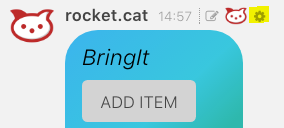
\includegraphics[scale=1.0]{Sections/3-HowToUse/Images/list_gear_icon.png}
  \caption{Button to show the available list's actions.}
\end{figure}

From the various options that are available, click on the one with the sharing icon.

% Inserire immagine dell'icona per condividere la lista
\begin{figure}[H]
  \centering 
  
\includegraphics[width=\textwidth]{Sections/3-HowToUse/Images/example.jpeg}
  \caption{Sharing button.}
\end{figure}

Once that the option has been clicked, the following popup will appear, showing the list of all the group that the list can be shared to.

% Inserire immagine del popup con la lista dei gruppi
\begin{figure}[H]
  \centering 
  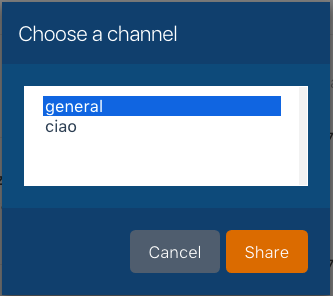
\includegraphics[scale=1.0]{Sections/3-HowToUse/Images/list_share_group.png}
  \caption{Popup showing the list of all the groups to which is possible sharing a list.}
\end{figure}

Now, select the group you want share the list with and then click on \textit{"Share"}. \\
This will open a new popup, letting you choose to which user you want to grant the \textbf{editor} permission. Once you have chose to which users to grant the permissions, click on \textit{"Ok"}.

% Immagine del popup con la lista degli utenti, alcuni selezionati
\begin{figure}[H]
  \centering 
  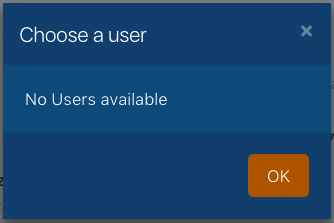
\includegraphics[scale=1.0]{Sections/3-HowToUse/Images/list_share_user.png}
  \caption{Popup to grant the editor permission to users inside the group.}
\end{figure}

%\subsection{[U] Forwarding a list}
In order to forward a list, hover on top of the bubble that represents the list and click on the gear icon.

% Inserire immagine delle opzioni che vengono fuori al passaggio del mouse sopra la bolla
\begin{figure}[H]
  \centering 
  
\includegraphics[width=\textwidth]{Sections/3-HowToUse/Images/example.jpeg}
  \caption{Button to show the available list's actions.}
\end{figure}

From the various options that will appear, click on the forward one.

% Inserire immagine icona di modifica della lista
\begin{figure}[H]
  \centering 
  
\includegraphics[width=\textwidth]{Sections/3-HowToUse/Images/example.jpeg}
  \caption{Icon of the option to forward a list.}
\end{figure}

Once that the option has been clicked, the following popup will appear, showing the list of all the group that the list can be forwarded to.

% Inserire immagine del popup con la lista dei gruppi
\begin{figure}[H]
  \centering 
  
\includegraphics[width=\textwidth]{Sections/3-HowToUse/Images/example.jpeg}
  \caption{Popup showing the list of all the groups to which is possible forwarding a list.}
\end{figure}

Now, select the group you want share the list with and then click on \textit{"Forward"}.